\documentclass[11pt,a4paper]{article}
\usepackage[margin=23mm,headheight=16pt]{geometry}
\usepackage[T1]{fontenc}
\usepackage{tgpagella}
\usepackage{amsmath,amssymb,amsthm,mathtools,bm,microtype,booktabs,tabularx,longtable,enumitem}
\usepackage{tikz}
\usetikzlibrary{arrows.meta,positioning,calc,patterns}
\usepackage{xcolor,fancyhdr,hyperref}
\definecolor{deepblue}{RGB}{25,50,99}
\definecolor{purple}{RGB}{104,69,170}
\definecolor{softblue}{RGB}{227,238,249}
\hypersetup{colorlinks=true,linkcolor=deepblue,urlcolor=deepblue}
\pagestyle{fancy}\fancyhf{}\fancyhead[L]{\small Quantum Gas Microscopy and Many-Body Reconstruction}\fancyhead[R]{\small Quantum Physics Companion VI}\fancyfoot[C]{\thepage}
\setlength{\parskip}{5pt}\setlength{\parindent}{0pt}
\setcounter{secnumdepth}{3}
\newtheorem{example}{Worked Example}
\newtheorem{remark}{Physical qualification}
\newcommand{\tr}{\operatorname{Tr}}
\newcommand{\kb}{k_{\mathrm B}}
\newcommand{\Var}{\operatorname{Var}}
\newcommand{\Cov}{\operatorname{Cov}}
\begin{document}
\begin{center}
{\Large\bfseries\color{deepblue} Quantum Gas Microscopy, Entanglement\\ Measurements and Many-Body Reconstruction}\par\medskip
{\large Chapter VI: Site-Resolved Rubidium Lattices, Correlations,\\ Renyi Entropies, SWAP Protocols and Tomographic Limits}\par\smallskip
{\small Advanced Quantum Physics Companion --- additive continuation, Chapters I--V unchanged}\par
\end{center}
\begin{abstract}
We develop the experimental and mathematical logic that connects fluorescence images of atoms in optical lattices to many-body observables. The distinction between a measured number configuration and a quantum wavefunction is maintained throughout. We derive density correlations, the static structure factor, parity-projection effects, site-resolved coherence, reduced density matrices, second Renyi entropy via two-copy SWAP measurements, and limits of partial tomography. Twelve worked examples, original diagrams and explicit experimental qualifications are included. Unless otherwise stated, orbitals here are \emph{motional modes of complete Rb-87 atoms}, not electronic $5s$ orbitals.
\end{abstract}
\tableofcontents\clearpage
\section{The experimental question: what can a microscope see?}
A Bose--Hubbard state on $L$ lattice sites may be written in a fixed-$N$ sector as
\begin{equation}|\Psi\rangle=\sum_{\mathbf n:\sum_i n_i=N}c_{\mathbf n}|n_1,\ldots,n_L\rangle.\label{eq:state}\end{equation}
A site-resolved microscope typically supplies an image from which an occupation estimate or parity pattern is inferred. It does not photograph the amplitudes $c_{\mathbf n}$ or their relative phases. Many identically prepared realizations are therefore required to estimate probability distributions and correlations. Quantum-gas microscopy links preparation, freezing the dynamics, fluorescence detection, image classification, repeated shots and statistical inference.
\begin{figure}[ht]\centering
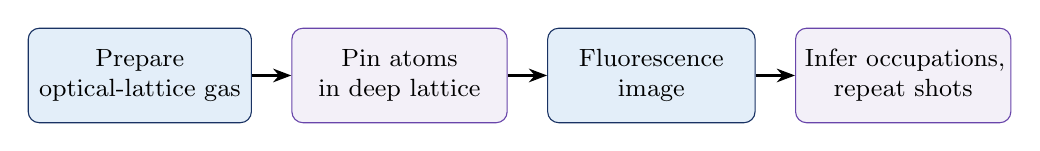
\begin{tikzpicture}[>=Stealth,node distance=5mm, every node/.style={font=\small}]
\node[draw=deepblue,rounded corners,fill=softblue,text width=2.6cm,align=center,minimum height=12mm] (a) {Prepare\\ optical-lattice gas};
\node[draw=purple,rounded corners,fill=purple!8,text width=2.5cm,align=center,minimum height=12mm,right=of a] (b) {Pin atoms\\ in deep lattice};
\node[draw=deepblue,rounded corners,fill=softblue,text width=2.4cm,align=center,minimum height=12mm,right=of b] (c) {Fluorescence\\ image};
\node[draw=purple,rounded corners,fill=purple!8,text width=2.5cm,align=center,minimum height=12mm,right=of c] (d) {Infer occupations,\\ repeat shots};
\draw[->,thick] (a)--(b);\draw[->,thick] (b)--(c);\draw[->,thick] (c)--(d);
\end{tikzpicture}
\caption{An idealized measurement pipeline. Imaging can be destructive, parity projected, or number resolving depending on the apparatus and cooling scheme.}
\end{figure}

\section{Optical lattice calibration and spatial resolution}
For counterpropagating lattice beams of wavelength $\lambda_L$ the intensity creates a periodic dipole potential, conventionally $V(x)=V_0\sin^2(k_Lx)$ with $k_L=2\pi/\lambda_L$ and spacing $a=\lambda_L/2$. Optical imaging has a diffraction scale $\delta x\sim\lambda_{\rm img}/(2\mathrm{NA})$ (a rule of thumb, not a universally exact resolution), so sites separated by $a$ can be challenging to resolve. High numerical aperture, fluorescence cooling, point-spread-function calibration and deconvolution are essential.
\begin{example}[Lattice spacing and nominal diffraction scale]
For $\lambda_L=1064\,\mathrm{nm}$, $a=532\,\mathrm{nm}$. For $\lambda_{\rm img}=780\,\mathrm{nm}$ and $\mathrm{NA}=0.8$, the simple diffraction scale is $\delta x\sim780/(1.6)=487.5\,\mathrm{nm}$. Since these scales are comparable, the precise point-spread function and site-lattice registration matter more than a crude binary ``resolved/unresolved'' rule.
\end{example}
\begin{figure}[ht]\centering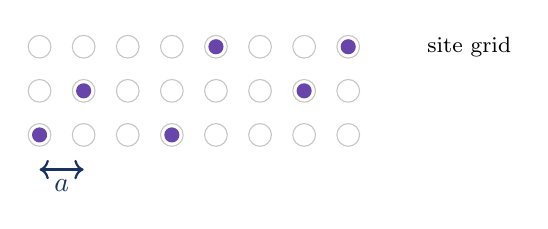
\begin{tikzpicture}[scale=.8]
\foreach \x in {0,...,7} {\foreach \y in {0,...,2} {\draw[gray!45] (\x*.7,\y*.7) circle (.18);}}
\foreach \x/\y in {0/0,1/1,3/0,4/2,6/1,7/2} {\fill[purple] (\x*.7,\y*.7) circle (.12);}
\draw[<->,deepblue,thick] (0,-.55)--node[below] {$a$} (.7,-.55);
\node[anchor=west,font=\footnotesize] at (6,1.4) {site grid};
\end{tikzpicture}\caption{A schematic reconstructed lattice configuration. Empty circles are possible sites, filled circles indicate inferred occupied sites.}\end{figure}
\section{Measurement operators: number-resolved versus parity detection}
An ideal projective number measurement at site $i$ has projectors $P_{n}^{(i)}=|n\rangle_i\langle n|$. The probability of outcome $n$ is $p_i(n)=\tr(\rho P_n^{(i)})$. A parity-sensitive channel instead reports $\pi_i=(-1)^{n_i}$, or equivalently the odd/even indicator $q_i=n_i\bmod2$. Light-assisted pair loss may cause an initially doubly occupied site to appear empty; it is not automatically faithful number resolution. Modern protocols can use alternative cooling or reconstruction to improve number resolution, but the experimental channel must be specified.
\begin{example}[Parity aliases distinct occupations]
The occupancies $n_i=0,2,4$ all have even parity, while $n_i=1,3,5$ have odd parity. Hence the configurations $(2,0,1)$ and $(0,2,1)$ produce identical parity strings $(0,0,1)$. A parity-only image cannot distinguish these physically different many-body outcomes.
\end{example}
\begin{example}[Occupation probability and measurement confusion]
Suppose a site is truly occupied with probability $p=0.7$, while false-negative and false-positive rates are $f_-=0.05$ and $f_+=0.02$. The observed occupation probability is $p_{\rm obs}=(1-f_-)p+f_+(1-p)=0.671$. Naively using $0.671$ as the true occupation gives a biased estimate; calibrated response matrices permit correction when invertible, with amplified statistical uncertainty.
\end{example}
\section{Estimating density profiles and connected correlations}
For measured site occupations $n_i^{(s)}$ from shot $s=1,\ldots,S$, the sample mean $\overline n_i=S^{-1}\sum_s n_i^{(s)}$ estimates $\langle n_i\rangle$. The connected correlator is
\begin{equation}C_{ij}=\langle n_i n_j\rangle-\langle n_i\rangle\langle n_j\rangle.\label{eq:cij}\end{equation}
For exact fixed atom number $\sum_i n_i=N$, one obtains $\sum_j C_{ij}=0$. Thus negative correlations between distinct sites may arise from number conservation alone and do not certify entanglement.
\begin{example}[Four measured configurations]
Consider four equally likely shots on three sites: $(1,1,0)$, $(1,0,1)$, $(0,1,1)$, $(1,1,0)$. Then $\langle n_1\rangle=3/4$, $\langle n_2\rangle=3/4$, and $\langle n_1n_2\rangle=1/2$. Therefore $C_{12}=1/2-9/16=-1/16$. The sample average with normalization $1/S$ is a plug-in estimator, whose finite-shot bias for products of estimated means should be considered in precision analysis.
\end{example}
\begin{example}[Binomial shot uncertainty]
For independent binary outcomes with success probability $p$, the standard error of the sample mean is $\sigma_{\widehat p}=\sqrt{p(1-p)/S}$. With $p=1/2$ and $S=1000$, this is about $0.0158$. Correlated shots or slow technical drifts invalidate the independent-identically-distributed assumption and can increase uncertainty.
\end{example}
\section{Static structure factor and collective correlations}
Define fluctuations $\delta n_j=n_j-\langle n_j\rangle$. For $L$ sites at positions $\mathbf R_j$, one common normalization is
\begin{equation}S(\mathbf q)=\frac{1}{L}\sum_{ij}e^{i\mathbf q\cdot(\mathbf R_i-\mathbf R_j)}\langle\delta n_i\delta n_j\rangle.\label{eq:sq}\end{equation}
Since $S(\mathbf q)=L^{-1}\langle|\sum_j e^{i\mathbf q\cdot\mathbf R_j}\delta n_j|^2\rangle\ge0$, it is nonnegative. In a fixed-$N$ ensemble, $S(0)=0$; the zero-momentum value depends on the ensemble and treatment of fluctuations.
\begin{example}[Perfect staggered density correlations]
Take a four-site ring, equally mixing configurations $(1,0,1,0)$ and $(0,1,0,1)$. Here $\langle n_j\rangle=1/2$, and $\delta n_j=\pm(-1)^j/2$ with a global random sign. At wavevector $q=\pi/a$, $\sum_j e^{iqja}\delta n_j=\pm2$, giving $S(\pi/a)=4/4=1$; at $q=0$ it vanishes. This is a classical mixture with strong density-order correlations, not by itself a proof of entanglement.
\end{example}
\section{Why site images do not directly measure first-order coherence}
The one-body density matrix is $\gamma_{ij}=\langle a_i^\dagger a_j\rangle$. Number snapshots in the site basis yield diagonal occupations and their moments but cannot, without additional manipulations or assumptions, determine off-diagonal $\gamma_{ij}$. One route to off-diagonal coherence is to release the gas and measure the momentum distribution:
\begin{equation}n(\mathbf k)\propto|\widetilde w(\mathbf k)|^2\sum_{ij}e^{i\mathbf k\cdot(\mathbf R_i-\mathbf R_j)}\gamma_{ij}.\end{equation}
Other options use interferometric beam-splitter operations on site modes or local basis rotations before readout. Such operations transform otherwise invisible phase information into measurable number statistics.
\begin{example}[Same number probabilities, different coherence]
Compare the coherent one-boson state $|+\rangle=(|10\rangle+|01\rangle)/\sqrt2$ with the incoherent mixture $\rho_{\rm mix}=\tfrac12(|10\rangle\langle10|+|01\rangle\langle01|)$. Both give $p(10)=p(01)=1/2$, yet $\langle a_L^\dagger a_R\rangle=1/2$ for $|+\rangle$ and $0$ for the mixture. Every direct occupation statistic is identical, demonstrating why density images alone cannot establish coherence.
\end{example}
\section{Reduced density matrices and two kinds of entropy}
For a bipartition into sites $A$ and $B$, we first trace out $B$ to obtain $\rho_A=\tr_B\rho$.\par The von Neumann entropy is $S_A=-\tr(\rho_A\ln\rho_A)$. The second R\'enyi entropy is
\begin{equation}\boxed{S_2(A)=-\ln\tr(\rho_A^2).}\label{eq:renyi}\end{equation}
For a \emph{pure global state}, nonzero $S_A$ or $S_2(A)$ means entanglement across the $A|B$ partition. For a mixed global state, subsystem entropy also reflects classical and thermal uncertainty. A single local reduced density matrix cannot generally distinguish the two without additional information.
\begin{example}[Pure entangled state versus classical mixture]
For $|\Phi\rangle=(|10\rangle+|01\rangle)/\sqrt2$, $\rho_L=\operatorname{diag}(1/2,1/2)$ and $S_2(L)=\ln2$. The mixture from the previous example has the \emph{same} $\rho_L$, the same purity $1/2$ and the same $S_2(L)$, but is separable in the site-mode tensor product. A purity measurement of $A$ alone is an entanglement witness only if global purity is established or appropriate stronger criteria apply.
\end{example}
\section{Two-copy SWAP measurement of second Renyi entropy}
Consider two identical, independently prepared copies, each described by $\rho$. The operator $\mathrm{SWAP}_A$ exchanges the states of subsystem $A$ between the copies. Then
\begin{equation}\boxed{\tr\big[(\rho\otimes\rho)\mathrm{SWAP}_A\big]=\tr(\rho_A^2)=e^{-S_2(A)}.}\label{eq:swap}\end{equation}
To prove this, trace out the two complementary $B$ subsystems, giving $\rho_A\otimes\rho_A$. The trace identity $\tr[(X\otimes Y)\mathrm{SWAP}]=\tr(XY)$ completes the proof. Beam-splitter operations between corresponding sites of the two copies can map SWAP eigenvalues onto measurable parity observables, subject to protocol-dependent control and detection assumptions.
\begin{figure}[ht]\centering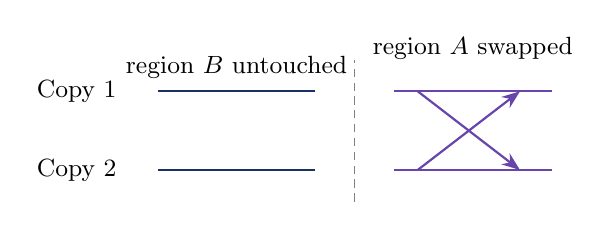
\begin{tikzpicture}[>=Stealth]
\node[font=\small,anchor=east] at (-.4,1) {Copy 1};\node[font=\small,anchor=east] at (-.4,0) {Copy 2};
\foreach \y in {0,1}{\draw[deepblue,thick] (0,\y)--(2,\y);\draw[purple,thick] (3,\y)--(5,\y);}
\draw[densely dashed,gray] (2.5,-.4)--(2.5,1.4);
\draw[->,purple,thick] (3.3,1)--(4.6,0);\draw[->,purple,thick] (3.3,0)--(4.6,1);
\node[font=\small] at (1,1.3) {region $B$ untouched};\node[font=\small] at (4,1.55) {region $A$ swapped};
\end{tikzpicture}\caption{Abstract two-copy SWAP operation on the chosen spatial region $A$. This is a logical diagram, not a specific microscope optical circuit.}\end{figure}
\begin{example}[Purity of the exact two-site/two-boson ground state]
Recall Chapter V: $|G\rangle=A(|20\rangle+|02\rangle)/\sqrt2+B|11\rangle$ with $A^2=(1-U/D)/2$, $B^2=(1+U/D)/2$, $D=\sqrt{U^2+16J^2}$. The left-site reduced state is $\operatorname{diag}(A^2/2,B^2,A^2/2)$ and its purity is
\begin{equation}\tr\rho_L^2=B^4+\frac{A^4}{2}.\end{equation}
At $U=0$, this is $3/8$, so $\boxed{S_2(L)=\ln(8/3)\approx0.98083}$. At $U/J\to\infty$, purity approaches $1$ and $S_2\to0$. A two-copy SWAP protocol could, in principle, measure precisely this purity.
\end{example}
\section{Randomized measurements and purity estimators}
Random local unitary transformations, followed by repeated projective measurements, can estimate subsystem purities under calibrated unitary ensembles. The reconstruction employs correlations between outcome probabilities across random bases. Different protocols require assumptions about sampling, readout errors, and local versus global randomization. A conceptual target is $\tr(\rho_A^2)$, but the estimator formula and sample complexity depend on the applied random-unitary ensemble and the local Hilbert-space dimension; it is misleading to claim a universal formula without specifying the protocol.
\section{Partial tomography and identifiability limits}
For a $d$-dimensional Hilbert space a general density matrix has $d^2-1$ independent real parameters. In the fixed-$N$ Bose--Hubbard sector, $d=\binom{N+L-1}{L-1}$. A single set of occupation-basis probabilities supplies only $d-1$ independent outcomes. Therefore no number of repeated images in that single basis suffices to reconstruct an arbitrary density matrix: additional noncommuting measurements or trustworthy model assumptions are required.
\begin{example}[Tomography counting for two atoms on three sites]
Here $d=\binom{4}{2}=6$. A general mixed density matrix therefore has $d^2-1=35$ real parameters. Occupation measurements in one basis give only $d-1=5$ independent probabilities. At least 30 additional independent constraints are needed to identify an arbitrary state; whether a proposed set of experimental basis rotations supplies them must be verified by its measurement map rank.
\end{example}
\begin{example}[Three-qubit analogy and informational completeness]
A single qubit density matrix is $\rho=(I+r_x\sigma_x+r_y\sigma_y+r_z\sigma_z)/2$. Measuring only $\sigma_z$ obtains $r_z$ and cannot identify $r_x$ or $r_y$. Measurements in $x,y,z$ bases can reconstruct the Bloch vector. Analogously, atomic lattice tomography requires changes of measurement basis to reveal coherences, not merely higher image counts in the same basis.
\end{example}
\section{Entanglement under particle-number superselection}
For identical particles the subsystem split is usually a split into spatial \emph{modes}. If local operations must conserve local particle number, coherences between distinct local-number sectors cannot necessarily be exploited as ordinary accessible entanglement. The fixed-$N$ state $(|10\rangle+|01\rangle)/\sqrt2$ has nonzero mode entropy, yet its operational entanglement under a strict local particle-number superselection rule requires careful resource accounting. Reference frames, multiple copies, or permitted operations change what can be accessed. We state explicitly which notion of entanglement is meant in each calculation.
\section{Finite temperature, imperfect detection and validation}
A real preparation is described by a density operator $\rho$ rather than necessarily a pure $|\Psi\rangle$. Photon scattering can heat atoms; imaging can lose atoms; two-copy protocols require independently calibrated copy equivalence and mode matching; number filtering and postselection can bias correlation functions. Essential validation includes (i) known-occupation calibration, (ii) point-spread-function registration, (iii) confusion matrix or parity response, (iv) drift diagnostics, (v) uncertainty intervals obtained from independent preparations, (vi) an explicit noise model for entropic estimates, and (vii) a report distinguishing directly measured quantities from reconstructed or model-dependent ones.
\section{A concrete reproducible analysis exercise}
Take an open chain of $L=4$ sites and $N=4$ bosons. Enumerate all $\binom{7}{3}=35$ Fock configurations. Build the Bose--Hubbard Hamiltonian by placing onsite terms $U\sum_i n_i(n_i-1)/2$ on the diagonal and nearest-neighbor hopping $-J\sqrt{(n_i+1)n_j}$ off diagonal. For each $U/J\in\{0,1,2,4,8,16\}$: diagonalize the exact matrix, calculate $\gamma_{ij}$, $C_{ij}$ and the half-chain reduced density matrix $\rho_{\{1,2\}}$; report $S_2$ and $S$, then simulate synthetic number snapshots and compare estimators with exact expectation values. Finally compare the pure ground state to a thermal Gibbs state $\rho_\beta=e^{-\beta H}/\tr(e^{-\beta H})$ at the same $U/J$, noting that nonzero subsystem entropy is not by itself entanglement in the mixed-state case.

\section{Detailed derivation: occupations, moments and finite-shot bias}
A microscope records a sequence of random variables $n_i^{(1)},\ldots,n_i^{(S)}$, not a deterministic density field. Define the raw estimators
\begin{equation}\widehat m_i=\frac1S\sum_{s=1}^{S}n_i^{(s)},\qquad \widehat m_{ij}=\frac1S\sum_{s=1}^{S}n_i^{(s)}n_j^{(s)}.\end{equation}
The obvious connected-correlation estimator $\widehat C^{\rm plug}_{ij}=\widehat m_{ij}-\widehat m_i\widehat m_j$ is biased even for independent identically distributed preparations. Indeed,
\begin{align}
\mathbb E[\widehat m_i\widehat m_j]&=\frac1{S^2}\left[S\mathbb E(n_in_j)+S(S-1)\mathbb E(n_i)\mathbb E(n_j)\right]\\
&=\frac1S\mathbb E(n_in_j)+\left(1-\frac1S\right)\mathbb E(n_i)\mathbb E(n_j).
\end{align}
Subtracting, we obtain $\mathbb E[\widehat C^{\rm plug}_{ij}]=(1-1/S)C_{ij}$. Thus an unbiased version is
\begin{equation}\boxed{\widehat C_{ij}=\frac{S}{S-1}\left(\widehat m_{ij}-\widehat m_i\widehat m_j\right),\quad S>1.}\end{equation}
The formula is valid for independent equivalent preparations with well-defined second moments. Bootstrapping independent shots can estimate uncertainties, but shots with common drifts require block resampling or an explicit time-series model.
\begin{example}[Finite-shot correction at $S=4$]
Using $\widehat C^{\rm plug}_{12}=-1/16$ from the four-shot example, the unbiased sample-covariance estimator is $\widehat C_{12}=(4/3)(-1/16)=-1/12$. These are different estimates from the same dataset; neither provides an error bar without a statistical model.
\end{example}
\section{Detailed derivation: the SWAP identity by indices}
Let $\{|i\rangle\}$ be an orthonormal basis of subsystem $A$. The swap operator acts as $W|i\rangle|j\rangle=|j\rangle|i\rangle$. Then for any $d\times d$ matrices $X,Y$,
\begin{align}
\tr[(X\otimes Y)W]
&=\sum_{ij}\langle i,j|(X\otimes Y)|j,i\rangle\\
&=\sum_{ij}X_{ij}Y_{ji}=\tr(XY).
\end{align}
For two copies of a bipartite density operator $\rho_{AB}$, trace over $B_1B_2$ and substitute $X=Y=\rho_A$. The identity gives Eq.~\eqref{eq:swap} exactly. Importantly, \emph{copy independence} is a premise: if the copies have correlations, $\rho\otimes\rho$ is not the correct input state.
\begin{example}[Unequal copies measure an overlap, not a purity]
If the prepared subsystem states are $\rho_A$ and $\sigma_A$, the same SWAP experiment yields $\tr(\rho_A\sigma_A)$. For pure qubit states $|0\rangle$ and $|1\rangle$, this is zero, even though each state's purity equals one. Therefore two-copy mismatch is not a small bookkeeping detail; it changes the quantity being estimated.
\end{example}
\section{Measurement basis rotations: a complete single-qubit analogue}
A qubit density matrix has the Bloch representation $\rho=(I+\vec r\cdot\vec\sigma)/2$. Suppose the experiment measures three Pauli expectation values $m_x=\langle\sigma_x\rangle$, $m_y=\langle\sigma_y\rangle$, $m_z=\langle\sigma_z\rangle$. Then
\begin{equation}\boxed{\rho=\frac12\begin{pmatrix}1+m_z&m_x-im_y\\m_x+im_y&1-m_z\end{pmatrix}.}\end{equation}
Physicality demands $m_x^2+m_y^2+m_z^2\le1$; finite sample noise may violate the bound, motivating constrained maximum-likelihood or Bayesian reconstruction. An analogous optical-lattice procedure needs a characterized family of control operations, a measurement map, and enough independent observables to span the chosen state model.
\begin{example}[Reconstructing a coherent superposition]
For $|+\rangle=(|0\rangle+|1\rangle)/\sqrt2$, the expectations are $(m_x,m_y,m_z)=(1,0,0)$ and $\rho=\tfrac12\bigl(\begin{smallmatrix}1&1\\1&1\end{smallmatrix}\bigr)$. A measurement restricted to the computational $z$ basis would return $(1/2,1/2)$ and cannot distinguish this state from $I/2$; including the $x$ basis resolves their difference.
\end{example}
\section{Microscopy versus interferometry: which operator is measured?}
Local fluorescence observation naturally approximates a measurement of site number $n_i=a_i^\dagger a_i$. After a coherent lattice beam splitter between sites $L,R$, the measured difference can become sensitive to off-diagonal coherence. Consider a 50:50 transformation $b_1=(a_L+a_R)/\sqrt2$, $b_2=(a_L-a_R)/\sqrt2$. Then
\begin{equation}b_1^\dagger b_1-b_2^\dagger b_2=a_L^\dagger a_R+a_R^\dagger a_L.\end{equation}
Thus a number-difference measurement \emph{after} the transformation estimates the real part of the original coherence. A controllable relative phase before mixing provides access to the imaginary part. This is a minimal mathematical example of converting phase into intensity or number information.
\begin{example}[Distinguishing coherent and incoherent one-atom states]
For $|+\rangle$, the transformed modes have outcomes $b_1$ occupied with unit probability and $b_2$ empty. For the incoherent mixture of $|10\rangle$ and $|01\rangle$, the same transformation yields a balanced output mixture. Both preparations had the same original site occupations. The additional controlled operation makes their otherwise hidden off-diagonal difference experimentally visible.
\end{example}
\section{A validated measurement program for a four-site rubidium chain}
The following sequence makes a realistic analysis plan, but does not assume that any specific laboratory apparatus supports every operation. First calibrate a deep-lattice fluorescence measurement on known one-atom sites, quantifying losses, false positives and parity projection. Second prepare a fixed-number four-site gas and acquire site images with shot time stamps. Third compare measured $\langle n_i\rangle$, $C_{ij}$, and $S(q)$ against exact diagonalization of the four-site Bose--Hubbard Hamiltonian. Fourth implement an additional basis rotation or interferometric measurement to access at least one off-diagonal $\gamma_{ij}$. Fifth, \emph{only if} sufficiently matched two-copy preparations and beam-splitter operations are available, measure a SWAP-based $S_2$ of a chosen spatial block. Sixth quantify thermal and detection biases with independent calibration data and report model mismatch rather than tuning the Hamiltonian parameters on the final test shots.

\begin{center}\small
\begin{tabularx}{\linewidth}{@{}p{3.2cm}X X@{}}\toprule
Observable & Measurement primitive & Main limitation \\ \midrule
$\langle n_i\rangle$ & Site-resolved occupancy & Detection confusion, loss \\
$C_{ij}$ & Repeat occupancy shots & Shot covariance, number conservation \\
$\gamma_{ij}$ & Interference / basis rotation & Phase calibration \\
$S_2(A)$ & Two-copy SWAP / random bases & Global purity, copy mismatch \\
Full $\rho$ & Informationally complete bases & Exponential parameter count \\
\bottomrule
\end{tabularx}
\end{center}
The experimental conclusion must be proportional to the evidence. A parity image supports parity distributions. Density snapshots support density correlations. Interferometric rotations support certain off-diagonal coherences. A validated copy protocol supports subsystem purity. None of these automatically establishes a complete many-body wavefunction.

\section{Further problems (with guidance)}
\begin{enumerate}[leftmargin=*,itemsep=4pt]
\item Show $\sum_j C_{ij}=0$ when total number is fixed. \emph{Hint:} correlate $\delta n_i$ with $\sum_j\delta n_j=0$.
\item Derive the intensity standing wave from two counterpropagating laser fields and determine lattice spacing.
\item Write the response matrix for binary site occupancy with false-positive/false-negative probabilities; solve for the true occupancy.
\item Construct two states with identical occupation probabilities but opposite relative phases; compare $\gamma_{LR}$.
\item Prove the SWAP trace identity for arbitrary finite-dimensional matrices $X,Y$ using a product basis.
\item Calculate $S_2$ of the left site at $U/J=4$ using exact coefficients from Chapter V.
\item Explain why a purity measurement of a subsystem does not necessarily certify entanglement if the global state is mixed.
\item Compute the static structure factor for two independent unit-filling sites with zero density fluctuations.
\item Enumerate all Fock basis configurations for $N=3,L=3$ and count their dimensions.
\item For $d=10$, compare the number of density matrix parameters with outcomes of one orthonormal basis measurement.
\item Design a calibration test to distinguish actual doublons from parity-projected imaging outcomes.
\item Show how two-copy copy-mismatch errors can alter the interpretation of a SWAP expectation.
\end{enumerate}
\section{Selected references and historical context}
\begin{enumerate}[leftmargin=*]
\item W. S. Bakr et al., ``A quantum gas microscope for detecting single atoms in a Hubbard-regime optical lattice,'' \emph{Nature} \textbf{462} (2009), 74--77.
\item J. F. Sherson et al., ``Single-atom-resolved fluorescence imaging of an atomic Mott insulator,'' \emph{Nature} \textbf{467} (2010), 68--72.
\item R. Islam et al., ``Measuring entanglement entropy in a quantum many-body system,'' \emph{Nature} \textbf{528} (2015), 77--83.
\item T. Brydges et al., ``Probing R\'enyi entanglement entropy via randomized measurements,'' \emph{Science} \textbf{364} (2019), 260--263.
\item C. Gross and I. Bloch, ``Quantum simulations with ultracold atoms in optical lattices,'' \emph{Science} \textbf{357} (2017), 995--1001.
\item M. Greiner et al., ``Quantum phase transition from a superfluid to a Mott insulator in a gas of ultracold atoms,'' \emph{Nature} \textbf{415} (2002), 39--44.
\item H. M. Wiseman and J. A. Vaccaro, ``Entanglement of Indistinguishable Particles Shared between Two Parties,'' \emph{Physical Review Letters} \textbf{91} (2003), 097902.
\end{enumerate}
\end{document}
